% Created 2017-01-07 Sat 00:45
\documentclass[a4paper]{article}
\usepackage[utf8]{inputenc}
\usepackage[T1]{fontenc}
\usepackage{fixltx2e}
\usepackage{graphicx}
\usepackage{grffile}
\usepackage{longtable}
\usepackage{wrapfig}
\usepackage{rotating}
\usepackage[normalem]{ulem}
\usepackage{amsmath}
\usepackage{textcomp}
\usepackage{amssymb}
\usepackage{capt-of}
\usepackage{hyperref}
\usepackage{amssymb,amsmath}
\usepackage{natbib}
\usepackage[margin=2cm]{geometry}
\usepackage{fancyhdr} %For headers and footers
\pagestyle{fancy} %For headers and footers
\usepackage{acronym}
\usepackage{fontspec}
\usepackage{lastpage} %For getting page x of y
\usepackage{float} %Allows the figures to be positioned and formatted nicely
\floatstyle{boxed} %using this
\usepackage{draftwatermark}
\restylefloat{figure} %and this command
\usepackage{url} %Formatting of yrls
\rhead{
\includegraphics[width=3cm]{berkeley}}
\chead{}
\lfoot{Draft}
\cfoot{}
\setlength{\parskip}{1em}
\rfoot{\thepage\ of \pageref{LastPage}}
\setmainfont{FreightSans Pro}
\acrodef{GHG}{Greenhouse Gas}
\acrodef{SLCP}{Short-Lived Climate Pollutants}
\acrodef{CAP}{Criteria Air Pollutants}
\acrodef{PM2.5}{Particulate Matter 2.5 $\mu$m}
\acrodef{NOX}{Oxides of Nitrogen}
\acrodef{CO2e}{Carbon Dioxide Equivalents}
\acrodef{CARB}{California Air Resources Board}
\acrodef{DF}{Displacement Factor}
\acrodef{FCP}{Forest Climate Plan}
\acrodef{BOF}{California Board of Forestry}
\acrodef{BC}{Black Carbon}
\acrodef{TC}{Total Carbon}
\acrodef{BOE}{California Board of Equalization}
\acrodef{TPO}{Timber Products Output}
\acrodef{OC}{Organic Carbon}
\author{Peter Tittmann, Ph.D.}
\date{\today}
\title{Emissions reductions from harvested wood products and management residuals}
\hypersetup{
 pdfauthor={Peter Tittmann, Ph.D.},
 pdftitle={Emissions reductions from harvested wood products and management residuals},
 pdfkeywords={},
 pdfsubject={},
 pdfcreator={Emacs 24.5.1 (Org mode 8.3.4)}, 
 pdflang={English}}
\begin{document}

\maketitle
\tableofcontents

\pagebreak

\thispagestyle{empty}

\listoffigures

\listoftables

\newpage

\pagenumbering{arabic}

\section{California Forest Management Emissions Profile}
\label{sec:orgheadline3}

Forest management activities in California produce logs for lumber markets while maintaining and enhancing forest health. In addition to merchantable logs, these harvest activities produce logging residuals that are either left in the stand to decompose, or pile burned as directed by forest practice rules (\href{http://calfire.ca.gov/resource_mgt/downloads/2013_FP_Rulebook_with_Tech_RuleNo1.pdf}{California Forest Practice Rules}, Article 7 §
917.2). The extent to which these residuals are utilized avoiding open combustion or decomposition materially impacts emissions of \ac{GHG} and \ac{SLCP}..

The majority of biomass produced from forest management activities end up as residual biomass material that is either left in the woods to decompose, or aggregated at a landing where it is eventually burned. When considered alongside the accumulation of woody material from historic fire suppression activity, there exists a heightened volume of combustible woody material in excess of historic reference conditions, elevating the risk of damaging wildfire in much of California’s forestland. Currently, common practice for fuel load management in California forests involves prescribed natural fire and sanitation pile burning. However, these approaches have limitations as previous studies have demonstrated that prescribed natural fire is often only effective at reducing fuel loading and maintaining fire resilient landscapes when it is coupled with mechanical treatment to remove biomass \cite{Stephens2009c}. Open pile burning of residual biomass can also result in greater emissions of strong radiative forcing agents (black carbon) and criteria air pollutants such as \ac{PM2.5} and \ac{NOX} when compared to controlled combustion in biomass power plants with modern emissions control technology. 

Ultimately, any combustion or decomposition of residual material results in emissions of \ac{GHG}, \ac{CAP}, and \ac{SLCP}. In the absence of forest management activity, atmospheric emissions are produced from stochastic processes such as wildfire, pest, and disease outbreaks. Utilization strategies are necessary to reduce the air quality impact of common forestry practice. The high climate opportunity cost\footnote{Climate opportunity cost is used in this context to refer to the aggregate emissions of particulate and gasses with strong radiative forcing properties associated with open pile or broadcast burning.} of open burning residual biomass in forestry and agriculture favor diverting residual material streams towards alternative utilization strategies such as biomass power. Figure \ref{fig:wood_fates} presents an overview of emissions and emissions reduction pathways for wood from California's forests. 

\begin{figure}[htb]
\centering
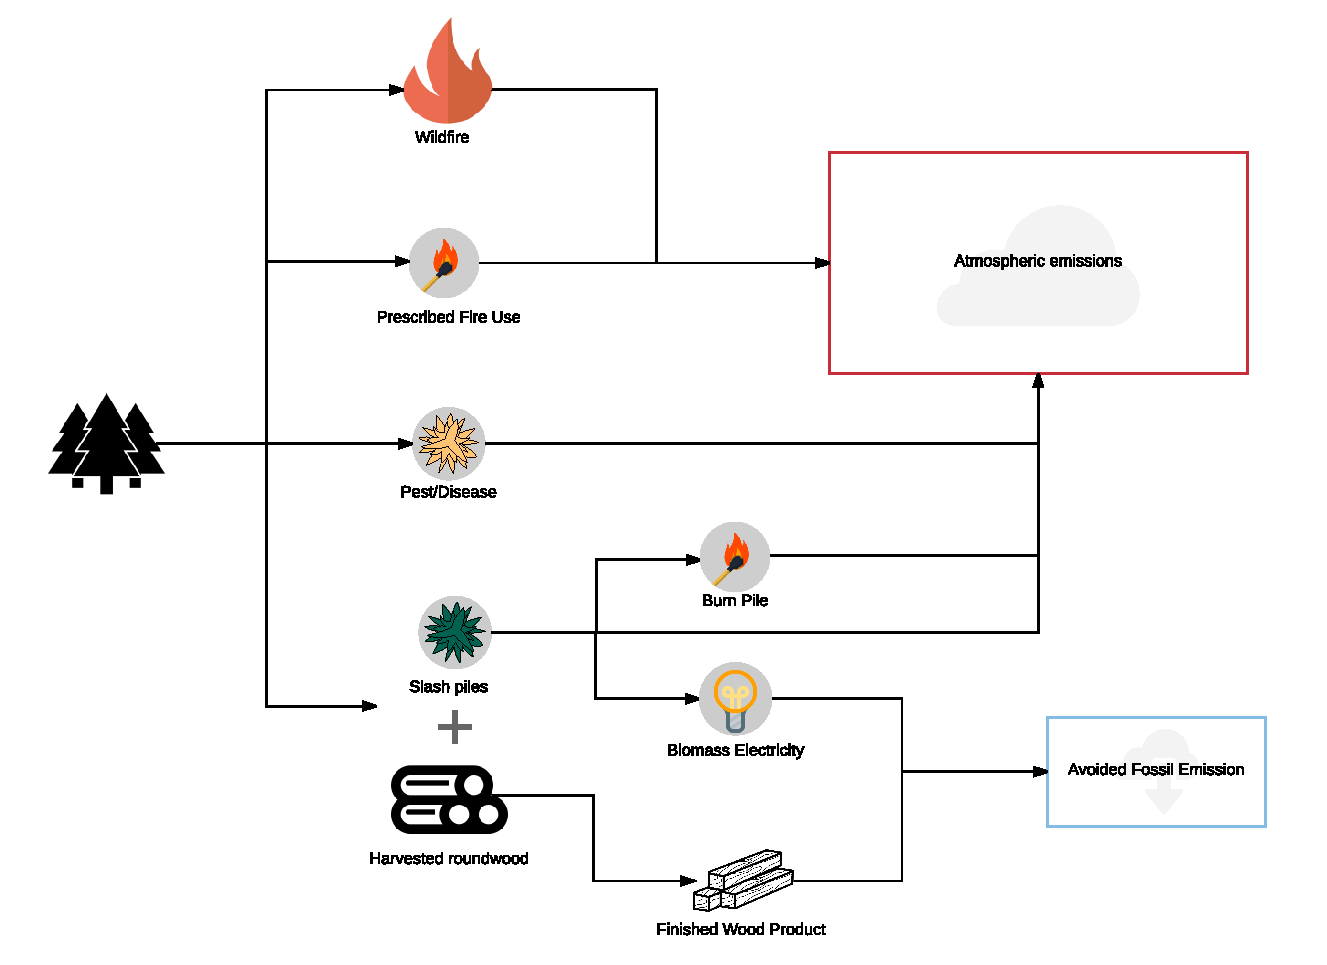
\includegraphics[width=0.75\textwidth]{./graphics/wood_fates_rs.pdf}
\caption{Overview of fates of wood resulting from harvest and mortality in California forests. Note that time is not represented in this figure. \label{fig:wood_fates}}
\end{figure}


The focus of this analysis is on deriving the net \ac{CO2e} emissions and emissions reductions associated with \textbf{management activity}. This report does not assess greenhouse gas emissions from pest or disease induced mortality, which is estimated at approximately 34 MMT of \ac{CO2e} annually in California forests \cite{Christensen2016}. Emissions from mortality are indirectly related to management activities just as wildfire is, and must be accounted for to comprehensively evaluate the climate impacts of harvesting. To estimate emissions and reductions by forest  management activity, it is necessary to take the following steps:

\begin{enumerate}
\item Estimate \ac{CO2e} emissions from burning forest management
residuals using the \ac{CARB}, \ac{CAP} and \ac{GHG} emissions inventories.

\item Estimate the volume and fate of wood that is removed, left in the
forest, and burned as a result of direct anthropogenic management
activities.

\item Applay life-cycle \ac{DF} for all utilized wood and apply \ac{DF} to harvested wood to obtain an aggregate estimate to estimate emissions reductions from wood use.
\end{enumerate}

\subsection{Report Objectives}
\label{sec:orgheadline1}

Quantifying the climate effects of wood products and forest management
residuals is important to the development of the \ac{FCP} \footnote{The \href{http://www.fire.ca.gov/fcat/}{Forest Climate Action Team} (FCAT) was assembled in August of 2014 with the primary purpose of developing a Forest Carbon Plan by the end of 2016. FCAT is comprised of Executive level members from many of the State’s natural resources agencies, state and federal forest land managers, and other key partners directly or indirectly involved in California forestry. FCAT is under the leadership of CAL FIRE, Cal-EPA, and The Natural Resources Agency.} as well as efforts underway by the \ac{BOF} and CalFire to meet the intent of AB 1504 (2010)\footnote{\href{http://leginfo.legislature.ca.gov/faces/billTextClient.xhtml?bill_id=200920100AB1504}{AB-1504} Forest resources: carbon sequestration.(2009-2010)}. To
inform these efforts, this report provides estimates of the following:

\begin{itemize}
\item Statewide \ac{GHG} and \ac{SLCP} emissions produced from the combustion or
decomposition of logging residuals.
\item Statewide \ac{GHG} emissions reductions from the use of wood products harvested in
the state.
\end{itemize}


Estimates are based empirical data and reflect past forest
management activities. It is \textbf{critical} to note that the empirical
data used in this analysis reflect point-in-time measures that are
affected by a dynamic system of climate, growth, and mortality as well as macroeconomic and policy forces. This analysis may provide insight into
opportunities to more effectively utilize woody biomass residuals from
current forest management activities to reduce emissions. 

\subsection{Key Findings}
\label{sec:orgheadline2}
\begin{itemize}
\item Baseline \ac{GHG} and \ac{SLCP} emissions from burning of forest
management residuals can be estimated and should be considered in
any forest management emissions baseline.

\item Average annual emissions from pile burning of logging residuals from roundwood harvesting
(including \ac{SLCP} and \ac{GHG} components) extrapolated from \ac{BOE} historical harvest data between 2000 and 2015 are estimated at \textbf{0.57 MMTCO2e}

\item Total annual emissions from pile burning of forest management residuals
(including \ac{SLCP} and \ac{GHG} components) extrapolated from CARB emissions
inventory are estimated at \textbf{2.5 MMTCO2e}

\item Wood harvested in California in 2012 resulted in avoided emissions of
\textbf{2.29 MMTCO2e}

\item Timber harvest producing roundwood including emissions from pile burning of logging residuals results in a net emissions reduction of \textbf{1.93 MMTCO2e}

\item Un-utilized slash from non-commercial management activities on National Forest System lands contributed emissions of \textbf{XXX MMTCO2e}

\item Forest Inventory and Analysis re-sample data has been used in the
southeast to quantify removals resulting from non-commercial
management activity and could be used for this purpose in California

\item The \href{https://ssl.arb.ca.gov/pfirs/}{Prescribed Fire Information Reporting System} (PFIRS) may be a useful tool for quantifying
emissions from pile burns and prescribed fire. It is a requirement that prescribed fires and pile
burns on National Forest System Lands are reported through PFIRS. However, California Air Quality Management
Districts are not required to report emissions through this system at this time. Therefore, it is not possible to associate burns in the PFIRS with commercial harvest activities.

\item Brown or \ac{OC} carbon has stronger radiative absorption than \ac{BC} and is associated with biomass burning. Accosting for anthropogenic production of \ac{OC} should be included in emissions baselines against which alternative utilization (energy) should be measured against.
\end{itemize}

\section{Estimating CO2 Equivalent Emissions from In-Forest Biomass Combustion}
\label{sec:orgheadline9}


The \ac{CARB} reports on emissions from in-forest biomass combustion with current \ac{GHG} and \ac{CAP} \href{http://www.arb.ca.gov/ei/ei.htm}{emissions inventories}. Both are necessary resources for establishing aggregate annual climate-forcing emissions (Figure \ref{fig:burn_diag}). 
The GHG inventory captures
gasses with radiative forcing properties including CO2 and CH4, but does not capture elemental
carbon or \ac{BC} emissions which also have strong radiative
forcing properties (Table \ref{tab:bc_gwp}). The \citet{CaliforniaAirResourcesBoard2015,CaliforniaAirResourcesBoard2016}
\ac{CAP} report captures \ac{SLCP} emissions from wildfire
(\texttt{80.52} MMTCO2e) and prescribed fire
(\texttt{3.66} MMTCO2e) from which black carbon emissions may be estimated. However, no reference in the CAP report is made to the source of these
SLCP estimates. When viewed in aggregate, a comprehensive reporting of total climate impact from anthropogenic burning may be estimated. 


\begin{figure}[htb]
\centering
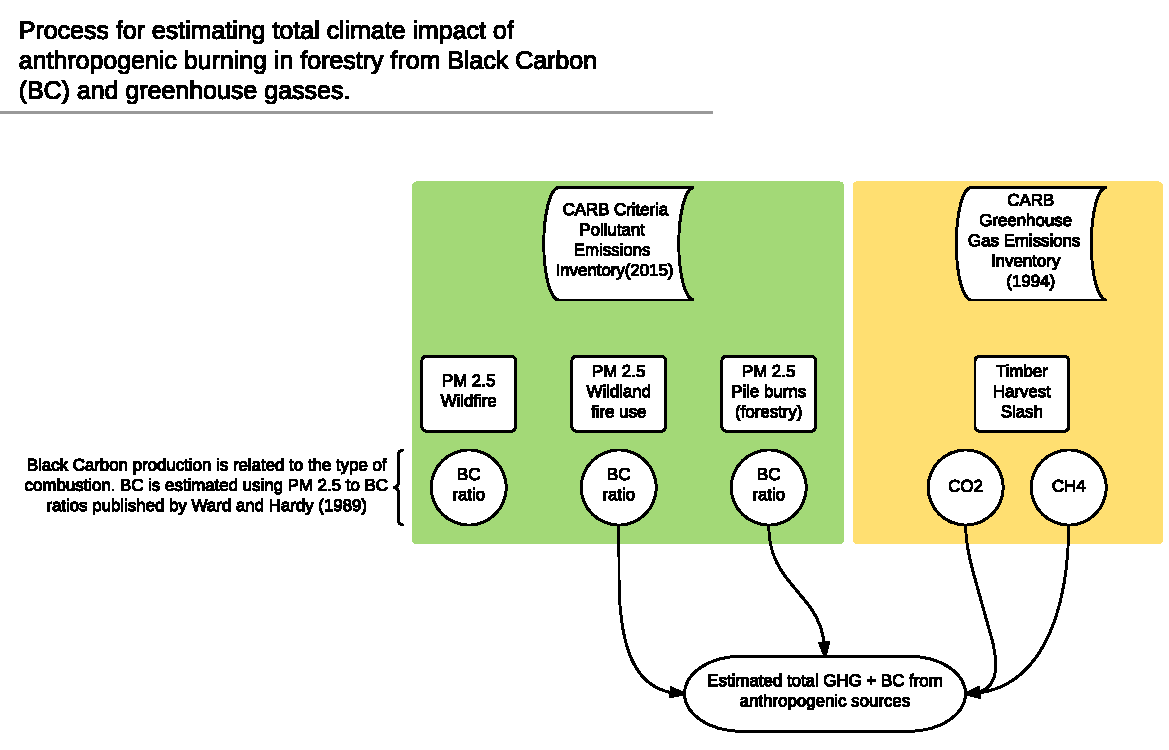
\includegraphics[width=0.75\textwidth]{./graphics/burning.pdf}
\caption{Data sources available from CARB for estimating \ac{GHG} and \ac{SLCP} emissions from forest management. \label{fig:burn_diag}}
\end{figure}

The \ac{GHG} inventory captures
gasses with radiative forcing properties including CO2 and CH4, but does not capture elemental
carbon or \ac{BC} emissions which also have strong radiative
forcing properties (Table \ref{tab:bc_gwp}). 

\begin{table}[htb]
\centering
\begin{tabular}{rrrrrrl}
GWP\(_{\text{20}}\) & GWP\(\sigma_{\text{20}}\) & GWP\(_{\text{100}}\) & GWP\(\sigma_{\text{100}}\) & GWP\(_{\text{500}}\) & GWP\(\sigma_{\text{500}}\) & Source\\
\hline
2200.0 & 888.82 & 633.33 & 255.41 & 193.33 & 77.67 & Fuglestvedt2010\\
3200.0 &  & 900.0 &  &  &  & CaliforniaAirResourcesBoard2015\\
\end{tabular}
\caption{Range of Global Warming Potential(GWP) values for Black Carbon.\label{tab:bc_gwp}}

\end{table}


The \citet{CaliforniaAirResourcesBoard2015,CaliforniaAirResourcesBoard2016}
\ac{CAP} report captures \ac{SLCP} emissions from wildfire
(\texttt{80.52} MMTCO2e) and prescribed fire
(\texttt{3.66} MMTCO2e) from which \ac{BC} emissions may be estimated. However, no reference in the \ac{CAP} report is made to the source of these
SLCP estimates. When viewed in aggregate, a comprehensive estimate of total climate impact from anthropogenic burning may be made. 

\subsection{Estimating biomass combustion from 'Forest Management' using the \ac{CARB} \ac{CAP} inventory.}
\label{sec:orgheadline4}

To estimate total biomass from \ac{PM2.5}, I assume 90\% consumption of biomass in piles and use the relationship of pile tonnage to PM emissions as calculated from the \href{http://depts.washington.edu/nwfire/piles/}{Piled Fuels Biomass and Emissions Calculator} provided by the Washington State Department of Natural Resources (Table \ref{pfbec}). This calculator is based on the \href{http://www.fs.fed.us/pnw/fera/research/smoke/consume/index.shtml}{Consume} fire behavior model published by the US Forest Service. 

\begin{table}[htb]
\centering
\begin{tabular}{lrrrrr}
Pile Type & Pile Biomass (tons) & Consumed Fuel (tons) & PM2.5 (tons) & CO2 (tons) & CH4 (tons)\\
\hline
Half sphere & 1.36018 & 1.22416 & 0.00826308 & 2.03664 & 0.00343071\\
\end{tabular}
\caption{\label{tab:orgtable1}
Ratios of biomass to \ac{GHG} emissions from the Piled Fuels Emissions Calculator and based on the CONSUME model.}

\end{table}


The ratio of \ac{PM2.5} to unburned tonnage used in this report are found in Table \ref{tab:pm_ratios}. 

\begin{table}[htb]
\centering
\begin{tabular}{lr}
Ratio & Value\\
\hline
\ac{PM2.5} \(\Delta\) Biomass & 164.60932\\
\end{tabular}
\caption{Ratio of piled biomass \ac{PM2.5} used in this report. \label{tab:pm_ratios}}

\end{table}


Using these ratios we then estimate biomass consumed based on reported \ac{PM2.5} emissions in the \ac{CARB} \ac{CAP} inventory (Table \ref{tab:cap_biomass})

\begin{table}[htb]
\centering
\begin{tabular}{rrr}
YEAR & PM2.5 (t) & Pile-Burned Biomass (t)\\
\hline
2000 & 5474.31 & 901129.28\\
2005 & 5474.31 & 901129.28\\
2010 & 5474.31 & 901129.28\\
2012 & 5477.3 & 901621.96\\
2015 & 5480.51 & 902150.69\\
\end{tabular}
\caption{Forest biomass burned in piles based on ARB-reported PM2.5 emissions in the 'Forest Management' category. \label{tab:cap_biomass}}

\end{table}

\subsection{Estimating biomass combustion from using the \ac{CARB} \ac{CAP} inventory.}
\label{sec:orgheadline5}
The estimate of biomass consumed in 'Forest 'Management' using this methodology far exceeds the total volume of biomass residuals produced from commercial timber harvesting in the state. Using the \ac{BOE} historical harvest data, logging residual production rates for commercial timber harvest from \cite{Morgan} and bioenergy consumption from \cite{Mciver2012} (Table \ref{tab:bio_vol}) we can estimate the volume of logging residuals produced.

\begin{table}[htb]
\centering
\begin{tabular}{rr}
year & Percent of roundwood harvest used in bioenergy\\
\hline
2000 & 2.4\\
2006 & 3.6\\
2012 & 8.2\\
\end{tabular}
\caption{\% volume of wood diverted to Bioenergy use by year \label{tab:bio_vol}}

\end{table}

The availability of data for bioenergy consumption of logging residuals does not allow us to precisely estimate the consumption for years other than reported by \cite{Mciver2012}. In this analysis, for years that bioenergy consumption is reported, I use that value. As the states biomass energy infrastructure began to consume substantial amounts of residual in the early 1980's \citep{Morris2000}, we assume that the average consumption from the 3 years reported is representative annual consumption. For years before 1980, we assume no bioenergy consumption.  This approach is less than ideal as there has been a great deal of variability in the appetite for logging residuals from biomass power plants. Un-utilized logging residues are estimated from logging residuals not used in bioenergy (Table \ref{tab:unused_lr}). These results are based on a normal probability distribution defined by an estimate (0.0615 cf logging residuals per cf of growing-stock removals) and a range (\textpm{} 0.00229 cf/cf) at the 95\% confidence interval for logging residual generation from roundwood harvest. This is one of several factors contributing to instances where bioenergy consumption is greater than logging residues  produced. Other factors include:

\begin{itemize}
\item Lack of temporal resolution in bioenergy consumption
\item Consumption by biomass power plants of in-woods residuals produced from forest management that did not result in commercial roundwood harvest
\end{itemize}


\begin{table}[htb]
\centering
\begin{tabular}{rrrr}
Year & Logging Residues & Bioenergy & Unutilized Logging Residuals\\
\hline
1978 & 1.37648 & 0 & 1.37648\\
1979 & 1.1869 & 0 & 1.1869\\
1980 & 0.732729 & 0.348909 & 0.38382\\
1981 & 0.552591 & 0.294654 & 0.257937\\
1982 & 0.0132148 & 0.255616 & -0.242402\\
1983 & 0.778638 & 0.370302 & 0.408337\\
1984 & 1.15256 & 0.391033 & 0.761526\\
1985 & 0.690508 & 0.421028 & 0.26948\\
1986 & 1.78313 & 0.470321 & 1.31281\\
1987 & 0.876609 & 0.496235 & 0.380373\\
1988 & 1.38311 & 0.514982 & 0.868128\\
1989 & 2.02822 & 0.487854 & 1.54036\\
1990 & 1.01987 & 0.443414 & 0.576451\\
1991 & 0.614629 & 0.352327 & 0.262302\\
1992 & 0.797516 & 0.327846 & 0.46967\\
1993 & 0.671715 & 0.316598 & 0.355117\\
1994 & 0.560554 & 0.255396 & 0.305158\\
1995 & 0.217133 & 0.254293 & -0.0371602\\
1996 & 0.602055 & 0.250654 & 0.351401\\
1997 & 0.581323 & 0.264659 & 0.316664\\
1998 & 0.472128 & 0.230584 & 0.241544\\
1999 & 0.454244 & 0.236429 & 0.217815\\
2000 & 0.189259 & 0.109927 & 0.0793326\\
2001 & 0.261365 & 0.17677 & 0.0845949\\
2002 & 0.0983162 & 0.186364 & -0.0880478\\
2003 & 0.191743 & 0.183387 & 0.00835635\\
2004 & 0.163134 & 0.188128 & -0.0249946\\
2005 & 0.452135 & 0.190224 & 0.261911\\
2006 & 0.218927 & 0.136793 & 0.0821336\\
2007 & 0.285568 & 0.179306 & 0.106261\\
2008 & 0.0783061 & 0.151297 & -0.0729905\\
2009 & 0.115737 & 0.088771 & 0.026966\\
2010 & 0.131594 & 0.128029 & 0.00356518\\
2011 & 0.161427 & 0.142034 & 0.019393\\
2012 & 0.0995951 & 0.249688 & -0.150093\\
2013 & 0.1313 & 0.181402 & -0.0501019\\
2014 & 0.188085 & 0.161662 & 0.0264229\\
\end{tabular}
\caption{Probabilistic disposition of logging residuals from roundwood harvest in CA. Volume in million bone-dry tons.}

\end{table}

In the absence of empirical data reflecting the actual combustion of logging residuals and considering that in much of the states timber producing region tree-length or log-length yarding methods are used which do not result in accumulation of logging residuals at a landing as is the case with whole-tree yarding, we might assume 50\% of the logging residuals not used in bioenergy would be burned in open piles per California Forest Practice Rules. 

\subsection{Estimating Black Carbon Emissions from Biomass Burning}
\label{sec:orgheadline6}

\acf{BC} is not directly reported by statewide emissions summaries.\ac{BC} is a fraction of the \ac{TC} component of \ac{PM2.5}. \ac{PM2.5} emissions are published annually by \ac{CARB} (\href{http://www.arb.ca.gov/ei/emissiondata.htm}{Criteria air pollutant (CAP) emissions estimates}). 
By using the 2015 CAP emissions estimates shown in Table \ref{tab:arb_pm_ann} with estimated ratios of 
smoldering to flaming combustion for hand/machine piled burns, prescribed 
natural fire and wildfire from \citet{Ward1989}, Black Carbon emissions
can be calculated from PM
2.5 with Eq. \eqref{eq-bc}


\begin{center}
\begin{tabular}{llr}
Source (\ac{CARB} nomenclature) & Description & \ac{PM2.5} (t y\(^{\text{-1}}\))\\
\hline
ALL VEGETATION & Wildfire & 137630.15\\
FOREST MANAGEMENT & Pile burning & 5480.51\\
WILDLAND FIRE USE (WFU) & Prescribed natural fire & 6802.43\\
\end{tabular}

\end{center}

Using the 2015 \ac{CAP} emissions estimates shown in Table \ref{tab:arb_pm_ann} with estimated ratios of smoldering to flaming combustion for hand/machine piled burns, prescribed natural fire and wildfire from \citet{Ward1989}, \ac{BC} emissions can be estimated from PM 2.5 using equation \eqref{eq-bc}


\begin{align}
BC &= \left( PM_{2.5} \times F \times TC_f \times BC_f\right) + \left( PM_{2.5} \times S \times TC_s \times BC_s\right) \label{eq-bc} \\
\text{where:} \nonumber \\
BC &= \text{Black Carbon (mass units)} \nonumber \\
PM_{2.5} &= PM_{2.5} \text{ (mass units)} \nonumber \\
F &= \text{Percent of combustion in flaming phase} \nonumber \\
TC_f &= \text{Total Carbon fraction of } PM_{2.5} \text{ for flaming phase} \nonumber \\
BC_f &= \text{Black Carbon fraction of Total Carbon for flaming phase} \nonumber \\
S &= \text{Percent of combustion in smoldering phase} \nonumber \\
TC_s &= \text{Total Carbon fraction of } PM_{2.5} \text{ for smoldering phase} \nonumber \\
BC_s &= \text{Black Carbon fraction of Total Carbon for smoldering phase} \nonumber
\end{align}

The ratio of smoldering to flaming combustion behavior for each biomass burning scenario means that each has a different \ac{BC} \(\Delta\) \ac{PM2.5}
ratio. To arrive at a rough estimate of \ac{BC} emissions based on PM2.5, ratios from  \citet{Ward1989} and \citet{Jenk1996} ratios in Table \ref{tab:bc_pm} are used herein.
\begin{table}[htb]
\centering
\begin{tabular}{llrrrrr}
Combustion & Context & TC t\(^{\text{-1}}\) \ac{PM2.5} & TC\(_{\text{Cv}}\) t\(^{\text{-1}}\) \ac{PM2.5} & BC t\(^{\text{-1}}\) TC & BC\(_{\text{Cv}}\) t\(^{\text{-1}}\) \ac{PM2.5} & OC t\(^{\text{-1}}\) TC\\
\hline
f & p & 0.621 & 0.07 & 0.023 & 0.15 & 0.598\\
s & p & 0.587 & 0.03 & 0.02 & 0.41 & 0.5675\\
f & wf & 0.608 & 0.09 & 0.1108 & 0.506 & 0.4976\\
s & wf & 0.641 & 0.08 & 0.045 & 0.29 & 0.59625\\
\end{tabular}
\caption{Factors used for calculating \ac{BC} emissions. Combustion refers to flaming (f) or smoldering(s) phases and context establishes if the ratio is used in on modeling emissions from wildfire (wf) or pile burns (p). \ac{BC} is a fraction of \ac{TC} which is a fraction of total \ac{PM2.5}. \ac{OC} is reported here for reference only. Coefficients of variation (C\(_{\text{v}}\)) are reported here as well. \label{tab:bc_pm}}

\end{table}

Given the variance in \ac{BC} production from smoldering (\textpm{} 15\%) and flaming (\textpm{} 41\%) phases (Table \ref{tab:bc_pm}), actual emissions of \ac{BC}  may vary substantially depending on combustion. In addition to these estimates \cite{Chow2010} provides an alternative source for estimates of \ac{BC} and \ac{OC} emissions in the state in 2006. Further work is necessary to evaluate the impacts of \ac{OC} on the net \ac{CO2e} emissions from pile burning. \cite{Pokhrel2016} estimated the absorptive properties of \ac{OC} to be 1.5 - 2.5 that of \ac{BC}. \cite{Chow2010} estimated that 29,530 Mt of \ac{OC} was emitted from wildfires in 2006. 

\subsection{Estimating \ac{GHG} Emissions from Biomass Burning}
\label{sec:orgheadline7}
The \ac{CARB} GHG emissions inventory resolved to combustion source (piles, prescribed, etc.) for forests and rangelands has not been updated since 2004. To provide a comparable estimate of GHG emissions from pile burning we use the ratio of \ac{PM2.5} to the net \ac{CO2e} emissions from all \ac{GHG} species produced from the Piled Fuels Eissions Calculator (CONSUME model equations) sources two approaches are taken. As \ac{PM2.5} is reported in the \ac{CAP} for pile burning we can apply this ratio to estimate \ac{GHG} emissions for the same time period.


To estimate \ac{GHG} emissions from \textbf{pile burning}, we use the ratio of
\ac{PM2.5} to CO2 and to CH4 from the Piled Fuels Emissions Calculator. These ratios are then applied to \ac{CARB}-reported \ac{PM2.5} emissions to estimate \ac{GHG} emissions (Table \ref{tab:pfe_calc}).


\ac{GHG} emissions from \textbf{wildfire and prescribed fire} are difficult to estimate at present but the
\href{http://www.arb.ca.gov/cc/inventory/archive/tables/net_co2_flux_2007-11-19.pdf}{\ac{CARB} \ac{GHG} emissions inventory} provided estimates for years between 1994 and 2004 (Table \ref{arb_ghg_2004}).

\begin{table}[htb]
\centering
\begin{tabular}{lr}
Source Category & Average annual emissions 1994-2004 MMt CO2e\\
\hline
Forest and rangeland fires & 2.02\\
Timber harvest slash & 0.16\\
\end{tabular}
\caption{Annual \ac{GHG} Emissions estimated from CARB \ac{GHG} emissions inventory \label{arb_ghg_2004}}

\end{table}

\subsection{Estimating Total Emissions from Biomass Burning}
\label{sec:orgheadline8}
\label{sec:pile_emissions}

To arrive at an annual estimate of total \ac{CO2e} emissions, we combine \ac{BC} emissions estimates from the \ac{CARB} \ac{CAP} Emissions Inventory with the  \href{http://www.fs.fed.us/pnw/fera/research/smoke/consume/index.shtml}{USFS CONSUME} model combustion ratios. Overall, this analysis demonstrates that substantial emissions from forest management residuals have been reported by CARB emissions inventories and that such inventories could be utilized to establish a baseline condition for \ac{CO2e} emissions from forest management (Table \ref{tab:pile_summary}). 

Total emissions resulting from \textbf{pile burned} forest management residuals
can then be derived for the two greenhouse gasses produced from pile
burning (CO2, CH4) and from BC (Table \ref{tab:arb_pm_ann}).

\begin{table}[htb]
\centering
\begin{tabular}{rlrrrrr}
Year & Emissions source & CO2 (t) & CH4 (tCO2e) & BC (tCO2e) & BC-h (tCO2e) & BC-l (tCO2e)\\
\hline
2000 & FOREST MANAGEMENT & 1.34928\,(+06) & 63639.8 & 6.21335\,(+06) & 7.18357\,(+06) & 5.31602\,(+06)\\
2005 & FOREST MANAGEMENT & 1.34928\,(+06) & 63639.8 & 6.21335\,(+06) & 7.18357\,(+06) & 5.31602\,(+06)\\
2010 & FOREST MANAGEMENT & 1.34928\,(+06) & 63639.8 & 6.21335\,(+06) & 7.18357\,(+06) & 5.31602\,(+06)\\
2012 & FOREST MANAGEMENT & 1.35002\,(+06) & 63674.6 & 6.21674\,(+06) & 7.18749\,(+06) & 5.31892\,(+06)\\
2015 & FOREST MANAGEMENT & 1.35081\,(+06) & 63712 & 6.22039\,(+06) & 7.19171\,(+06) & 5.32204\,(+06)\\
\end{tabular}
\caption{\label{tab:orgtable2}
Emissions of \ac{SLCP} and \ac{GHG} from the 'Forest Management' \ac{CAP} \ac{PM2.5} emissions inventory. \label{tab:ghg_slcp}}

\end{table}

Table \ref{tab:ghg_slcp} reflects emissions from all biomass combustion meeting the definition of 'Forest Management'. It us useful in addition to understand the contribution that logging residuals from commercial timber harvesting make to this total.

\begin{table}[htb]
\centering
\begin{tabular}{rrrrrrr}
\% burned & LR burned (MBDT) & PM2.5 (t) & CO2 (t) & CH4 (tCO2e) & BC (tCO2e) & Total c\{CO2e\}\\
\hline
0.25 & 12502.3 & 75.9516 & 18720.2 & 882.951 & 86205.1 & 105808\\
0.5 & 80239.3 & 487.453 & 120145 & 5666.73 & 553260 & 679071\\
0.75 & 160479 & 974.906 & 240290 & 11333.5 & 1.10652\,(+06) & 1.35814\,(+06)\\
\end{tabular}
\caption{\label{tab:orgtable3}
Three emissions scenarios for pile burning of logging residuals from timber harvesting based on average annual harvest (2000 - 2015).}

\end{table}


The total \ac{CO2e} emissions from pile burning forestry residuals as reported by \ac{CARB} and pile burning logging residuals from roundwood harvesting from \ac{BOE} historical data are shown in Table \ref{tab:pile_summary}.


\begin{center}
\begin{tabular}{rl}
MMt CO2e & Source\\
\hline
1.4133952 & \ac{CO2e} \ac{GHG} pile burning\\
6.21335 & \ac{CO2e} \ac{BC}  pile burning\\
7.18357 & \ac{CO2e} \ac{BC}  pile burning  -- high\\
5.31602 & \ac{CO2e} \ac{BC}  pile burning  -- high\\
\hline
7.6199244 & \textbf{Total MMt CO2e -- Forest Management}\\
929052 & \textbf{Total MMt CO2e -- Timber Harvesting}\\
\end{tabular}
\label{tab:orgtable4}


\end{center}
These emissions are substantial and represent a significant opportunity to increase emissions reduction already realized from forestry. Ensuring that piled biomass from forest management activities are chipped and used in energy applications could eliminate up to 83\% (7.18 MMT \ac{CO2e}) of these emissions. It is important to note, however, that this estimate derived from the \ac{CAP} inventory implies that more than twice the total volume of logging residuals produced from commercial roundwood harvesting was burned in the context described by 'Forest Management' in the \ac{AP} inventory. While some of the difference here can be explained by the burning of residuals produced from non-commercial management activities, it is unlikely that the the full compliment of burned residuals from non-commercial activity is approximately the same as the total volume of loggin residuals produced from commercial roundwood harvest. As the \ac{CAP} inventory is based on reporting from local air districts it would seem that the margin of error in the \ac{CAP} estimate of \ac{PM2.5} emissions could be substantial.

\section{Estimating Emissions Impact from Utilization of Harvested Wood}
\label{sec:orgheadline20}
Wood harvested from California's forests are utilized in a variety of construction,
landscaping, and consumer products. During the manufacture of these products, this wood is fractionated 
through a multi-stage process of harvesting, processing, and utilization to reside in several residual biomass fates (below). 

\begin{description}
\item[{Logging Residuals}] Tops, limbs, and sub-merchantable material produced from harvest activities in the woods. These residuals may be left on site to naturally decompose or disposed of by anthropogenic pile burning or wildfire.
\item[{Processing (Mill) Residuals}] Sawdust, shavings, bark, and off cuts from primary and secondary manufacturing. These residuals may be directed towards alternative product streams (i.e. wood pellet, wood chip, power and heat generation) or sent to a landfill.
\item[{Construction Debris}] Fraction of wood used in construction or finished products that are not integrated into its final form. These residuals are most commonly sent to a landfill.
\item[{Demolition}] Wood used in construction that has reached the end of its useful life. These residuals are most commonly sent to a landfill.
\end{description}

These biomass fates have widely variable time horizons for the return of fixed carbon to the atmosphere. The extent to to which harvested wood is utilized can greatly influence the net emissions impact attributed to the initial forest management activity. While wood products used in construction, finished products, or other stable environments may sequester carbon for a long period, residues sent to landfills or left in the woods as slash emit climate forcing gasses to the atmosphere. Some of these wood residues may be redirected towards alternative controlled combustion applications (i.e., pellet production, power and heat generation)to avoid emissions.

Ultimately the fate of these pools are determined by a highly dynamic political and economic system. To understand how policy decisions will impact the fate and subsequent climate impact of harvested wood products, a detailed process model is necessary to track the distribution of harvested wood material. Figure \ref{wood_fates}

\subsection{Disposition of Harvested Wood in California.}
\label{sec:orgheadline15}
To provide a rough estimate of the fate of annually harvested roundwood material, we estimate the volume of wood biomass residing in logging, processing, and construction residuals. To estimate current values, we apply known milling efficiency improvements, logging utilization rates, and construction use efficiency to historical production volumes. 
\subsubsection{Logging Residues}
\label{sec:orgheadline10}
According to \citet{Morgan}, logging residues produced from sawlog harvest can be estimated using a factor of 0.0302 (+/-.0123 @95\%CI) times the total cubic sawlog volume delivered to a mill. \citet{Simmons2014} found that logging utilization has decreased in Idaho from 1990 to 2011 by 72\%. Unfortunately, we cannot say how logging residue production has changed over time in California. For the purpose of this analysis, we will assume that similar changes have occurred in California timber harvesting. 

We estimate logging residue production factor for years before 1990 based on the following equation. We assume 1990 residue ratios for all years prior.


\begin{align*}
V\llap{--}lr_{x} = V\llap{--}rw_{x}\left(\eta_{04}+\left(\eta_{o4}\eta_\Delta\right)\right)\\
\text{Where:}\\
V\llap{--}rw_{x} = \text{Rundwood volume harvested in year }x\\
\eta_{04} = \mathcal{N}(0.0302,0.0123) \text{ ratio of logging residues to roundwood harvested in CA, 2004}\\
\eta_\Delta = 0.72 \text{ (percent change in efficiency over time period)}\\
\end{align*}

For logging residue production factors between 1990 and 2004, we calculate logging residues by adjusting the logging residual ratio reported by \citet{Morgan} with the percent change in logging residual ratios estimated for Idaho by \citet{Simmons2014}. To reflect the uncertainty in the estimate provided by \citet{Morgan}, we estimate the logging residual using a randomly selected value from a normal probability distribution defined by the estimate and upper and lower bounds of the 95\% confidence interval provided:


\begin{align*}
V\llap{--}lr_{x} = V\llap{--}rw_{x}\left(\eta_{04}+ \left(\eta_{04}\left(\left(Y_1-x\right)\frac{\eta_\Delta}{Y_\Delta}\right)\right)\right)\\
\text{Where:}\\
V\llap{--}rw_{x} = \text{Roundwood volume harvested in year }x\\
\eta_{04} = \mathcal{N}(0.0302,0.0123) \text{ ratio of logging residues to roundwood harvested in CA, 2004}\\
Y_1 = 2004 \text{ (year for which logging residual estimate available for CA)} \\
x = \text{year for which logging residues are calculated}\\
\eta_\Delta = 0.72 \text{ (percent change in logging residue ratio over time period)}\\
Y_\Delta = 21\text{ (number of years over which logging residue ratio decreased)}
\end{align*}

Logging residual volume in years following 2004 are calculated as follows:

\begin{align*}
V\llap{--}lr_{x} = V\llap{--}rw_{x}\left(\eta_{04}- \left(\eta_{04}\left(\left(x-Y_1\right)\frac{\eta_\Delta}{Y_\Delta}\right)\right)\right)\\
\text{Where:}\\
V\llap{--}rw_{x} = \text{Rundwood volume harvested in year }x\\
\eta_{04} = \mathcal{N}(0.0302,0.0123) \text{ ratio of logging residues to roundwood harvested in CA, 2004}\\
Y_1 = 2004 \text{ (year for which logging residual estimate available for CA)} \\
x = \text{year for which logging residues are calculated}\\
\eta_\Delta = 0.72 \text{ (percent change in logging residue ratio over time period)}\\
Y_\Delta = 21\text{ (number of years over which logging residue ratio decreased)}
\end{align*}

\subsubsection{Processing Residues}
\label{sec:orgheadline11}
Milling efficiency has increased by roughly 14\% in California in the period between 1970 and 2006 \citet{Keegan2010}. For this analysis we assume a continuous improvement such that for years prior to 1970, milling efficiency in year \(x\) is calculated as:


\begin{align*}
V\llap{--}mr_{x} = V\llap{--}rw_{x} \left(\eta_{70}-\left((Y_1-x)\frac{\eta_\Delta}{Y_\Delta}\right\right)\\
\text{Where:}\\
V\llap{--}rw_{x} = \text{Rundwood volume harvested in year }x\\
\eta_{70} = 0.42 \text{ (milling efficiency in 1970)}\\
Y_1 = 1970 \text{ (earliest year mill efficiency available for)} \\
x = \text{year for which milling residues are calculated}\\
\eta_\Delta = 0.06\text{ (increase in milling efficiency from 1970-2011)}\\
Y_\Delta = 41\text{ (number of years overwhihc milling efficiency increased)}
\end{align*}

For years after 1970, milling efficiency for year \(x\) is calculated as:

\begin{align*}
V\llap{--}mr_{x} = V\llap{--}rw_{x} \left(\eta_{70}+\left((x-Y_1)\frac{\eta_\Delta}{Y_\Delta}\right\right)\\
\text{Where:}\\
V\llap{--}rw_{x} = \text{Rundwood volume harvested in year }x\\
\eta_{70} = 0.42 \text{ (milling efficiency in 1970)}\\
Y_1 = 1970 \text{ (earliest year mill efficiency available for)} \\
x = \text{year for which milling residues are calculated}\\
\eta_\Delta = 0.06\text{ (increase in milling efficiency from 1970-2011)}\\
Y_\Delta = 41\text{ (number of years overwhihc milling efficiency increased)}
\end{align*}

\subsubsection{Construction Residues}
\label{sec:orgheadline12}
To estimate annualized construction waste material, we apply the ratio of construction and demolition debris to finished wood products from \citet{McKeever2004} to roundwood harvest volumes from the \ac{BOE} (\cite{CaliforniaStateBoardofEqualization2015}). In 2002, construction debris was estimated as approximately 15\% of the total wood used in construction. Of note is that the data from \citeauthor{McKeever2004} is sparse and should be considered unreliable for years other than those for which it is reported. 

\subsubsection{Demolition Debris}
\label{sec:orgheadline13}
Debris from wood produced from wood grown on California forestland is outside of the scope of this report.

\subsubsection{Harvested Wood Residue Summary}
\label{sec:orgheadline14}
The following Table \ref{tab:me_and_lr} presents ten year average estimates of logging and milling residuals, finished lumber, and construction debris based on \ac{BOE} roundwood harvest volumes.

\begin{longtable}{rrrrrrr}
10-year start & 10-year end & RW & LR & MR & FL & CD\\
\hline
\endfirsthead
\multicolumn{7}{l}{Continued from previous page} \\
\hline

10-year start & 10-year end & RW & LR & MR & FL & CD \\

\hline
\endhead
\hline\multicolumn{7}{r}{Continued on next page} \\
\endfoot
\endlastfoot
\hline
1978 & 1988 & 681.701 & 71.2062 & 299.522 & 382.179 & 57.3269\\
1979 & 1989 & 680.582 & 70.0131 & 300.229 & 380.353 & 57.0529\\
1980 & 1990 & 681.083 & 85.4163 & 301.528 & 379.555 & 56.9333\\
1981 & 1991 & 681.601 & 80.9655 & 302.612 & 378.989 & 56.8483\\
1982 & 1992 & 686.631 & 85.6518 & 305.606 & 381.025 & 57.1538\\
1983 & 1993 & 695.872 & 61.338 & 310.422 & 385.451 & 57.8176\\
1984 & 1994 & 678.459 & 59.5059 & 303.4 & 375.059 & 56.2589\\
1985 & 1995 & 657.737 & 64.8848 & 294.892 & 362.845 & 54.4267\\
1986 & 1996 & 631.918 & 53.8304 & 284.093 & 347.825 & 52.1738\\
1987 & 1997 & 600.752 & 55.9357 & 270.919 & 329.833 & 49.4749\\
1988 & 1998 & 560.495 & 62.1744 & 253.572 & 306.923 & 46.0384\\
1989 & 1999 & 518.282 & 53.7261 & 235.308 & 282.975 & 42.4462\\
1990 & 2000 & 477.206 & 34.9406 & 217.442 & 259.764 & 38.9645\\
1991 & 2001 & 436.798 & 31.2871 & 199.72 & 237.078 & 35.5618\\
1992 & 2002 & 411.648 & 28.5456 & 188.838 & 222.81 & 33.4214\\
1993 & 2003 & 389.756 & 33.309 & 179.386 & 210.37 & 31.5555\\
1994 & 2004 & 370.287 & 23.5758 & 171.013 & 199.274 & 29.8912\\
1995 & 2005 & 360.411 & 20.2482 & 166.982 & 193.429 & 29.0143\\
1996 & 2006 & 349.131 & 22.3163 & 162.271 & 186.86 & 28.0291\\
1997 & 2007 & 338.319 & 20.1057 & 157.756 & 180.563 & 27.0845\\
1998 & 2008 & 321.14 & 20.4011 & 150.231 & 170.909 & 25.6364\\
1999 & 2009 & 299.649 & 19.3104 & 140.54 & 159.109 & 23.8663\\
2000 & 2010 & 283.222 & 15.1886 & 133.256 & 149.966 & 22.4949\\
2001 & 2011 & 271.892 & 16.5729 & 128.347 & 143.545 & 21.5318\\
2002 & 2012 & 266.945 & 15.0393 & 126.396 & 140.549 & 21.0823\\
2003 & 2013 & 266.193 & 12.2908 & 126.488 & 139.705 & 20.9558\\
2004 & 2014 & 262.901 & 13.9031 & 125.34 & 137.561 & 20.6341\\
\caption{Ten-year average logging and mill residual estimates based on BOE harvest volumes in Million Cubic Feet (MCF). RW:Roundwood harvested, LR: Logging residues, MR: Mill Residues, FL: Finished Lumber, CD: Construction Debris}
\\
\end{longtable}

\subsection{Emissions from Un-Utilized Residues}
\label{sec:orgheadline16}
\label{sec:boe_lr_emiss}

Residuals not utilized in bioenergy applications or sent to a landfill eventually 
produce emissions through combustion or biological decomposition of the
material over time. Most of these residues originate from logging activity.  
To calculate \ac{CO2e} emissions from unutilized residues, I first estimate the total volume of biomass  pile burned in forests using the \ac{CARB} estimate of \ac{PM2.5} (Section \ref{sec:pile_emissions}). 

To establish the fraction of logging residue that is left to decompose, one needs to know the volume of residues burned and used in bioenergy. 
To estimate the emissions from decomposition of logging residuals that are not burned, an estimate of consumption of biomass in pile burns would be necessary. In theory, the \ac{CARB} \ac(CAP\} inventory could provide an estimate using the ratio of \ac{PM} to biomass consumed. However the \ac{CARB}-derived pile burn estimate far exceeds the volume of logging residuals from the \ac{BOE} historical harvest data (Table \ref{tab:pile_bio_comparison})

\begin{table}[htb]
\centering
\begin{tabular}{rr}
\ac{CARB} estimate (BDT) & \ac{BOE} estimate (BDT)\\
\hline
901423.23 & 576008.93\\
\end{tabular}
\caption{Comparison of annual pile-burned biomass from forestry by \ac{CARB} with \ac{BOE}-derived estimate of loggin residuals produced from timber harvest.}

\end{table}

This is likely due to in part to the fact that the \ac{CARB} estimate includes non-commercial forest management activity.

\subsection{Emissions of Residuals from non-commercial managenent Activity}
\label{sec:orgheadline18}

The Timber Products Output (TPO) in California does not report wood volume produced from
non-commercial management activities. This includes management
activities such as pre-commercial thinning, sanitation thinning, and
fuels reduction thinning. Robust estimates for volume of removals from these sources are very difficult to obtain. In this report we only estimate unutilized residuals from public lands. The USFS Forest Service Activity Tracking System (FACTS) reports management activities conducted on National Forest System Lands. To ensure estimates of biomass volume using FACTS are not duplicative of reported volume in the TPO a series of filters are applied to the FACTS attributes to identify only non-commercial management activities.

\begin{enumerate}
\item Forest Service Activity Tracking System (FACTS)
\label{sec:orgheadline17}

Data from TPO does not account for forest management activities that do
not result in commercial products (timber sales, biomass sales). The
USFS
\href{http://data.fs.usda.gov/geodata/edw/datasets.php?dsetParent=Activities}{reports}
Hazardous Fuels Treatment (HFT) activities as well as Timber Sales (TS)
derived from the FACTS database. I use these two data sets to estimate
the number of acres treated that did not produce commercial material
(sawlogs or biomass) and where burning was not used. The first step is
to eliminate all treatments in the HFT data set that included timber
sales. I accomplish this by eliminating all rows in the HFT data set
that have identical \texttt{FACTS\_ID} fields in the TS dataset. I further
filter the HFT dataset by removing any planned but not executed
treatments (\texttt{nbr\_units1 >0} below -- \texttt{nbr\_units1} references
\texttt{NBR\_UNITS\_ACCOMPLISHED} in the USFS dataset, see metadata for HFT
\href{http://data.fs.usda.gov/geodata/edw/edw_resources/meta/S_USA.Activity_HazFuelTrt_PL.xml}{here}),
and use text matching in the 'ACTIVITY' and 'METHOD' fields to remove
any rows that contain reference to 'burning' or 'fire'. Finally, we
remove all rows that that reference 'Biomass' in the method category as
it is assumed that this means material was removed for bioenergy.I use a
range of 10-35 BDT/acre (mean 22.5) to convert acres reported in FACTS to volume.
The following table presents descriptive statistics for estimates of
residual unutilized wood biomass on an annual basis in million cubic
feet.

\begin{center}
\begin{tabular}{lrrrrr}
 & NFNC & NFC & P & FI & OP\\
\hline
count & 11 & 4 & 4 & 4 & 4\\
mean & 12.0194 & 17.7 & 28.95 & 66.425 & 2.4\\
std & 4.68948 & 5.07346 & 16.1593 & 6.07639 & 1.79444\\
min & 2.37421 & 11.2 & 11.2 & 59.6 & 0.3\\
25\% & 8.92407 & 15.025 & 19.525 & 62.225 & 1.275\\
50\% & 13.3557 & 18.5 & 27.75 & 66.85 & 2.5\\
75\% & 14.5349 & 21.175 & 37.175 & 71.05 & 3.625\\
max & 17.8532 & 22.6 & 49.1 & 72.4 & 4.3\\
\end{tabular}
\label{tab:orgtable5}


\end{center}
\begin{enumerate}
\item \textbf{Private industrial timber lands:} CalFIRE's
\href{http://www.calfire.ca.gov/resource_mgt/resource_mgt_forestpractice_gis}{Forest
Practice Geographical Information System}. \textbf{TODO}
\end{enumerate}
\end{enumerate}

\subsection{Avoided Emissions from Wood Product Displacement Factors}
\label{sec:orgheadline19}

For each product application, wood may be substituted by a range of other materials. For example, in
residential construction, precast concrete and structural steel framing
are competitive alternatives to wood. This choice of materials has a profound impact on \ac{GHG} emissions in the
construction sector and is expressed as a displacement
factor (DF). A displacement factor quantifies the amount of emissions
reduction achieved per unit of wood used. The displacement factors published in
\citep{Sathre2010} and used in this analysis are based on the
following emission reduction sources:

\begin{enumerate}
\item \textbf{Reduced emissions from manufacturing:} Wood products require less total
energy than to manufacture than products made from alternative materials.
\item \textbf{Avoided process emissions:} Production of wood alternatives such as cement are associated with 
substantial CO2 emissions.
\item \textbf{Carbon storage in products:} Carbon in harvested wood is drawn from
the atmosphere through photosynthesis and will remain fixed through
the useful life of the wood product.
\item \textbf{Carbon storage in forests:} Forests producing wood continue to grow.
It is assumed that forests producing wood in California are managed
to sustain forest growth (not converted to non-forest land uses).
\item \textbf{Avoided fossil fuel emissions due to bioenergy substitution:}
Logging and milling residuals used to produce energy avoid emissions
from fossil energy sources in the energy sector.
\item \textbf{Carbon dynamics in landfills:} A fraction of carbon from wood
deposited in landfills remains in semi-permanent storage.
The remainder is converted to methane through biological
decomposition in the landfill. Capture and use of the methane as an
energy source, in turn reduces emissions from fossil energy sources.
\end{enumerate}

A meta analysis conducted by \citep{Sathre2010} compared empirical analysis from 21 international studies and found an
average emissions reduction of 2.1 tons of carbon (3.9 t CO2e) per ton
of dry wood used. While studies ranged substantially around the average, the
authors found that the majority of published displacement factors ranged
between 1 and 3 tC/t dry wood. 

//** Displacement Factors Applied to Timber Products Output

To evaluate the climate impact of harvested wood in California, I used
harvested roundwood estimates from the Timber Products Output (TPO)
database\footnote{Timber Products Output Reporting Tool \href{http://srsfia2.fs.fed.us/php/tpo_2009/tpo_rpa_int1.php}{\url{http://srsfia2.fs.fed.us/php/tpo_2009/tpo_rpa_int1.php}}}. I used two estimates of the DF applied
to the harvested wood reported in the TPO based on whether logging
residuals were used in bioenergy or left in the woods (to decompse or
burn).

Figure \ref{fig:flow_chart} reflects the flow of wood
from Californias forest to its fate in-use and is the frame of
reference for the following analysis.

\begin{figure}[htb]
\centering
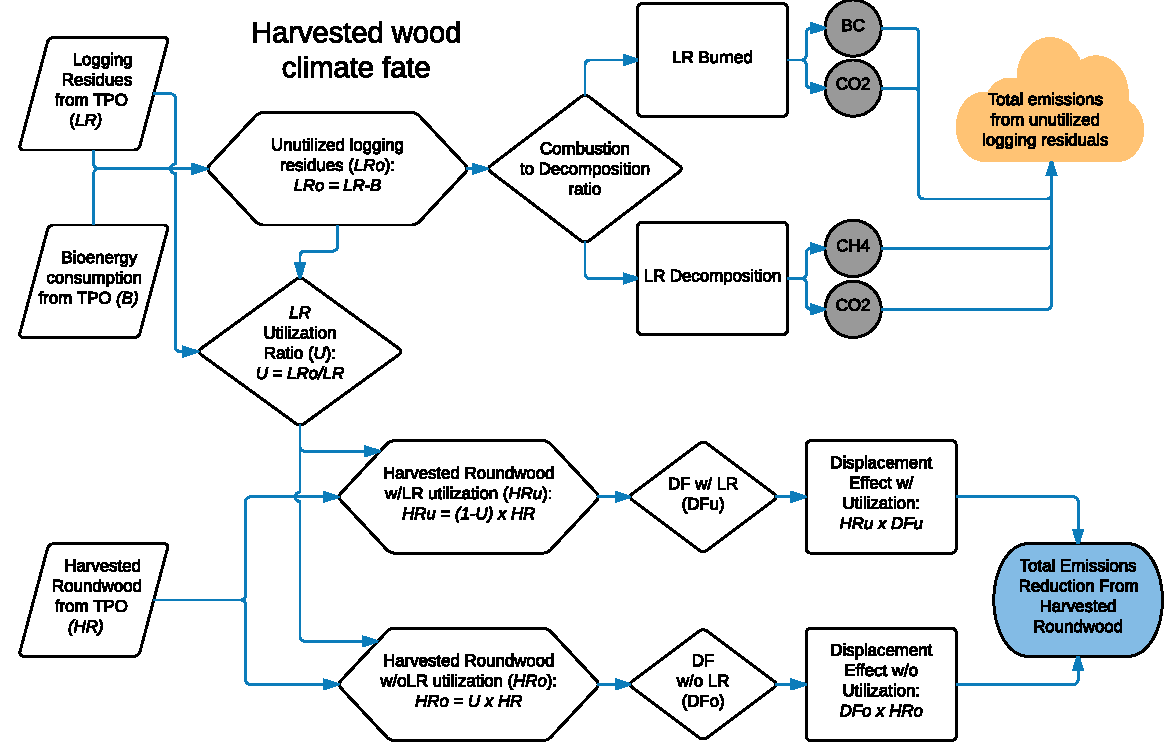
\includegraphics[width=0.75\textwidth]{./graphics/flow_chart.pdf}
\caption{Wood flows from timber harvest in California \label{fig:flow_chart}}
\end{figure}

I applied displacement factors reported by \cite{Sathre2010} to the
reported harvest volumes from the TPO database. 


The following references are used to
arrive at an average displacement factor of \textbf{2.625} tCO2e/t finished
wood product for harvested roundwood without
logging residue utilization.

\begin{table}[htb]
\centering
\begin{tabular}{lr}
reference & displacement factor\\
\hline
\citet{Eriksson2007} & 1.7\\
\citet{Eriksson2007} & 2.2\\
\citet{Salazar2009} & 4.9\\
\citet{Werner2005} & 1.7\\
\end{tabular}
\caption{Wood displacement factor without residue utilization \label{tab:df_no_use}}

\end{table}

For harvested roundwood with logging residue utilization the following
studies are used. I used an average of the DF reported here of \textbf{3.243} tCO2e/t finished
wood product.


\begin{table}[htb]
\centering
\begin{tabular}{lr}
reference & displacement factor\\
\hline
\citet{Eriksson2007} & 1.9\\
\citet{Eriksson2007} & 2.5\\
\citet{Gustavsson2006a} & 4\\
\citet{Gustavsson2006a} & 5.6\\
\citet{Gustavsson2006a} & 2.2\\
\citet{Gustavsson2006a} & 3.3\\
\citet{Pingoud2001} & 3.2\\
\end{tabular}
\caption{Wood discplacement factor with residue utilization \label{tab:df_inc_use}}

\end{table}



The TPO reports values in terms of roundwood harvested for products, but the
displacement factors presented in Sathre and O'Connor are in terms of
tons of carbon in wood products. Therefore we must assume a milling
efficiency to convert TPO volume estimates to finished wood product volume. I assumed
a milling efficiency of 0.5.


Further, TPO is reported in cubic feet and the DF implies a mass
unit. To convert cubic meters to a mass unit, we used the average wood
density of harvested volume in California weighted by species as reported 
in \citet{Mciver2012}. The resulting weighted average wood density used here is \textbf{27.94
lbs/cuft}.


We use the fraction of harvested roundwood used in bioenergy from \cite{Mciver2012} (Table \ref{tab:bio_vol})  to determine the percent of harvested wood used in bioenergy feedstocks. From personal communications with
\href{http://www.bber.umt.edu/staff/mciver.asp}{Chelsea McIver}, all bioenergy feedstock reported is sourced in-woods (ie, not mill residues).


\begin{center}
\begin{tabular}{rlrrr}
 & Ownership & Roundwood Products & Logging Residues & Year\\
\hline
0 & National Forest & 72.4 & 20.7 & 2012\\
1 & Other Public & 16.2 & 3.4 & 2012\\
2 & Forest Industry & 328.9 & 72.4 & 2012\\
3 & Other Private & 53 & 11.2 & 2012\\
4 & National Forest & 52.8 & 16.3 & 2006\\
5 & Other Public & 1.1 & 0.3 & 2006\\
6 & Forest Industry & 274.3 & 59.6 & 2006\\
7 & Other Private & 139.2 & 33.2 & 2006\\
8 & National Forest & 90.8 & 22.6 & 2000\\
9 & Other Public & 5.2 & 1.6 & 2000\\
10 & Forest Industry & 372.5 & 70.6 & 2000\\
11 & Other Private & 159.4 & 49.1 & 2000\\
12 & National Forest & 132.1 & 11.2 & 1994\\
13 & Other Public & 24.7 & 4.3 & 1994\\
14 & Forest Industry & 396.1 & 63.1 & 1994\\
15 & Other Private & 174.7 & 22.3 & 1994\\
\end{tabular}

\end{center}


In addition to the TPO, the California Board of Equalization (BOE) also
reports historic timber harvest volumes.  Comparing between years where both
sources report data, the BOE database reports on average, 8\% less volume than the TPO (Table \ref{tab:tpo_boe}) database. This is reasonable considering that:
\begin{enumerate}
\item BOE data may be under-reported, as there may be a financial incentive to reduce tax burden
\item BOE does not include volume harvested from native American tribal lands in the state
\end{enumerate}

\begin{longtable}{rrrr}
year & McIver, et. al. (2012) MMBF & BOE MMBF & BOE/M\&M\\
\hline
\endfirsthead
\multicolumn{4}{l}{Continued from previous page} \\
\hline

year & McIver, et. al. (2012) MMBF & BOE MMBF & BOE/M\&M \\

\hline
\endhead
\hline\multicolumn{4}{r}{Continued on next page} \\
\endfoot
\endlastfoot
\hline
1978 & 4606.0 & 4491 & 0.98\\
1979 & 4044.0 & 3991 & 0.99\\
1980 & 3478.0 & 3164 & 0.91\\
1981 & 2832.0 & 2672 & 0.94\\
1982 & 2488.0 & 2318 & 0.93\\
1983 & 3638.0 & 3358 & 0.92\\
1984 & 3701.0 & 3546 & 0.96\\
1985 & 4093.0 & 3818 & 0.93\\
1986 & 4416.0 & 4265 & 0.97\\
1987 & 4667.0 & 4500 & 0.96\\
1988 & 4847.0 & 4670 & 0.96\\
1989 & 4699.0 & 4424 & 0.94\\
1990 & 4264.0 & 4021 & 0.94\\
1991 & 3439.0 & 3195 & 0.93\\
1992 & 3192.0 & 2973 & 0.93\\
1993 & 3041.0 & 2871 & 0.94\\
1994 & 2814.0 & 2316 & 0.82\\
1995 & 2520.0 & 2306 & 0.92\\
1996 & 2515.0 & 2273 & 0.9\\
1997 & 2640.0 & 2400 & 0.91\\
1998 & 2420.0 & 2091 & 0.86\\
1999 & 2429.0 & 2144 & 0.88\\
2000 & 2244.0 & 1966 & 0.88\\
2001 & 1801.0 & 1603 & 0.89\\
2002 & 1691.73 & 1690 & 1.0\\
2003 & 1667.95 & 1663 & 1.0\\
2004 & 1704.0305 & 1706 & 1.0\\
2005 & 1738.5 & 1725 & 0.99\\
2006 & 1960.35 & 1631 & 0.83\\
2007 & 1759.6 & 1626 & 0.92\\
2008 & 1476.0745 & 1372 & 0.93\\
2009 & 911.19 & 805 & 0.88\\
2010 & 1302.38 & 1161 & 0.89\\
2011 & 1432.5 & 1288 & 0.9\\
2012 & 1421.3 & 1307 & 0.92\\
\caption{Total annual harvest reported by \citet{Mciver2012} and California Board of Equalization.\label{tab:tpo_boe}}
\\
\end{longtable}

// move to appendix?//The TPO reports harvest from tribal lands, which produces an average 0.74\% of the total
annual harvest in the state for the 37 years of parallel data. For
this analysis we used TPO data to include harvest volume from tribal lands. 


\begin{longtable}{rrrrr}
year & State & Federal & Private & Tribal\\
\hline
\endfirsthead
\multicolumn{5}{l}{Continued from previous page} \\
\hline

year & State & Federal & Private & Tribal \\

\hline
\endhead
\hline\multicolumn{5}{r}{Continued on next page} \\
\endfoot
\endlastfoot
\hline
1947 & 0.0 & 0.0 & 569.85 & 0.0\\
1948 & 0.0 & 0.0 & 735.29 & 0.0\\
1949 & 0.0 & 0.0 & 698.53 & 0.0\\
1950 & 0.0 & 0.0 & 808.82 & 0.0\\
1951 & 0.0 & 0.0 & 900.74 & 0.0\\
1952 & 2.57 & 113.79 & 808.82 & 4.78\\
1953 & 3.31 & 117.65 & 977.94 & 2.76\\
1954 & 2.94 & 141.54 & 880.51 & 4.6\\
1955 & 2.57 & 191.73 & 906.25 & 6.07\\
1956 & 4.41 & 206.99 & 862.13 & 5.33\\
1957 & 4.96 & 170.59 & 801.47 & 6.62\\
1958 & 5.51 & 208.27 & 821.69 & 6.99\\
1959 & 4.96 & 279.6 & 788.6 & 9.19\\
1960 & 5.15 & 250.37 & 680.15 & 8.82\\
1961 & 5.33 & 259.74 & 707.72 & 10.11\\
1962 & 6.25 & 259.01 & 744.49 & 8.64\\
1963 & 4.04 & 311.76 & 678.31 & 9.93\\
1964 & 4.6 & 348.16 & 643.38 & 9.01\\
1965 & 5.7 & 363.05 & 591.91 & 9.74\\
1966 & 5.88 & 360.85 & 545.96 & 8.27\\
1967 & 6.43 & 355.51 & 562.5 & 7.54\\
1968 & 8.82 & 440.44 & 542.28 & 14.52\\
1969 & 7.35 & 372.61 & 529.41 & 9.93\\
1970 & 6.25 & 345.4 & 481.62 & 5.15\\
1971 & 7.17 & 383.09 & 476.1 & 12.87\\
1972 & 6.8 & 411.58 & 591.91 & 12.13\\
1973 & 6.07 & 371.69 & 516.54 & 9.38\\
1974 & 7.35 & 322.79 & 525.74 & 9.38\\
1975 & 6.43 & 287.87 & 498.16 & 3.31\\
1976 & 7.35 & 348.53 & 507.35 & 6.99\\
1977 & 5.15 & 323.35 & 544.12 & 6.99\\
1978 & 5.15 & 332.35 & 509.19 & 8.64\\
1979 & 4.78 & 321.32 & 417.28 & 8.82\\
1980 & 3.68 & 279.04 & 356.62 & 7.72\\
1981 & 2.76 & 201.65 & 316.18 & 4.04\\
1982 & 7.72 & 173.9 & 275.74 & 1.47\\
1983 & 7.9 & 313.42 & 347.43 & 2.57\\
1984 & 6.25 & 288.05 & 386.03 & 3.86\\
1985 & 6.62 & 339.52 & 406.25 & 0.92\\
1986 & 5.33 & 365.26 & 441.18 & 4.96\\
1987 & 7.72 & 364.89 & 485.29 & 7.54\\
1988 & 5.7 & 403.68 & 481.62 & 2.57\\
1989 & 6.8 & 373.53 & 483.46 & 2.02\\
1990 & 4.41 & 283.09 & 496.32 & 2.57\\
1991 & 6.99 & 248.35 & 376.84 & 4.41\\
1992 & 4.23 & 190.99 & 391.54 & 5.88\\
1993 & 6.25 & 137.32 & 415.44 & 2.39\\
1994 & 3.12 & 152.02 & 362.13 & 2.76\\
1995 & 7.35 & 101.1 & 354.78 & 2.94\\
1996 & 10.11 & 86.4 & 365.81 & 2.39\\
1997 & 8.64 & 101.65 & 375.0 & 2.76\\
1998 & 4.78 & 83.46 & 356.62 & 2.94\\
1999 & 0.0 & 97.24 & 349.26 & 0.0\\
2000 & 3.49 & 63.42 & 345.59 & 1.84\\
2001 & 2.94 & 56.07 & 272.06 & 1.84\\
2002 & 0.18 & 31.38 & 279.41 & 2.5\\
2003 & 0.18 & 28.85 & 277.57 & 3.29\\
2004 & 0.18 & 20.78 & 292.28 & 3.05\\
2005 & 0.18 & 43.66 & 275.74 & 1.95\\
2006 & 0.74 & 41.61 & 318.01 & 2.37\\
2007 & 0.18 & 58.57 & 264.71 & 3.55\\
2008 & 0.18 & 37.7 & 233.46 & 2.48\\
2009 & 0.18 & 30.37 & 136.95 & 0.72\\
2010 & 0.18 & 49.89 & 189.34 & 1.79\\
2011 & 0.18 & 55.42 & 207.72 & 2.1\\
2012 & 5.13 & 37.39 & 218.75 & 1.49\\
\caption{Annual harvest by ownership from \citet{Mciver2012} (MCF)\label{tab:MandM}}
\\
\end{longtable}

To use the TPO data to estimate emissions reductions using the DF, we apply a
conversion factor of \textbf{5.44} MCF/MMBF. This is an approximation as the
actual sawlog conversion factor varies with average harvested log size, which has changed over time.  


Using the ratio of logging residuals consumed by bioenergy (mciver), to the total logging residuals reported in the TSP, we can calculated the harvest volume the ratio of harvest volume to logging residuals used in bioenergy,
we calculateted 
based on the ratio of reported consumption of logging residuals in
bioenergy by \citeauthor{Mciver2012} to the total logging residuals reported
in the TPO. \citeauthor{Mciver2012} report bioenergy consumption from 2000
forward. For years previous, we use the average bioenergy consumption
from 2000 -- 2012. These results assume bioenergy consumption
throughout the reporting years. Bioenergy use of residuals did not
begin until the late 1970. Further analysis is necessary to modify
these results to reflect the development of the bioenergy industry.

To calculate the total emissions reduction resulting from California's
timber harvest, we apply the appropriate displacement factor (with or
without logging residual utilization) to the commensurate fraction of
harvested roundwood. The results are shown in the following chart.

\begin{figure}[htb]
\centering
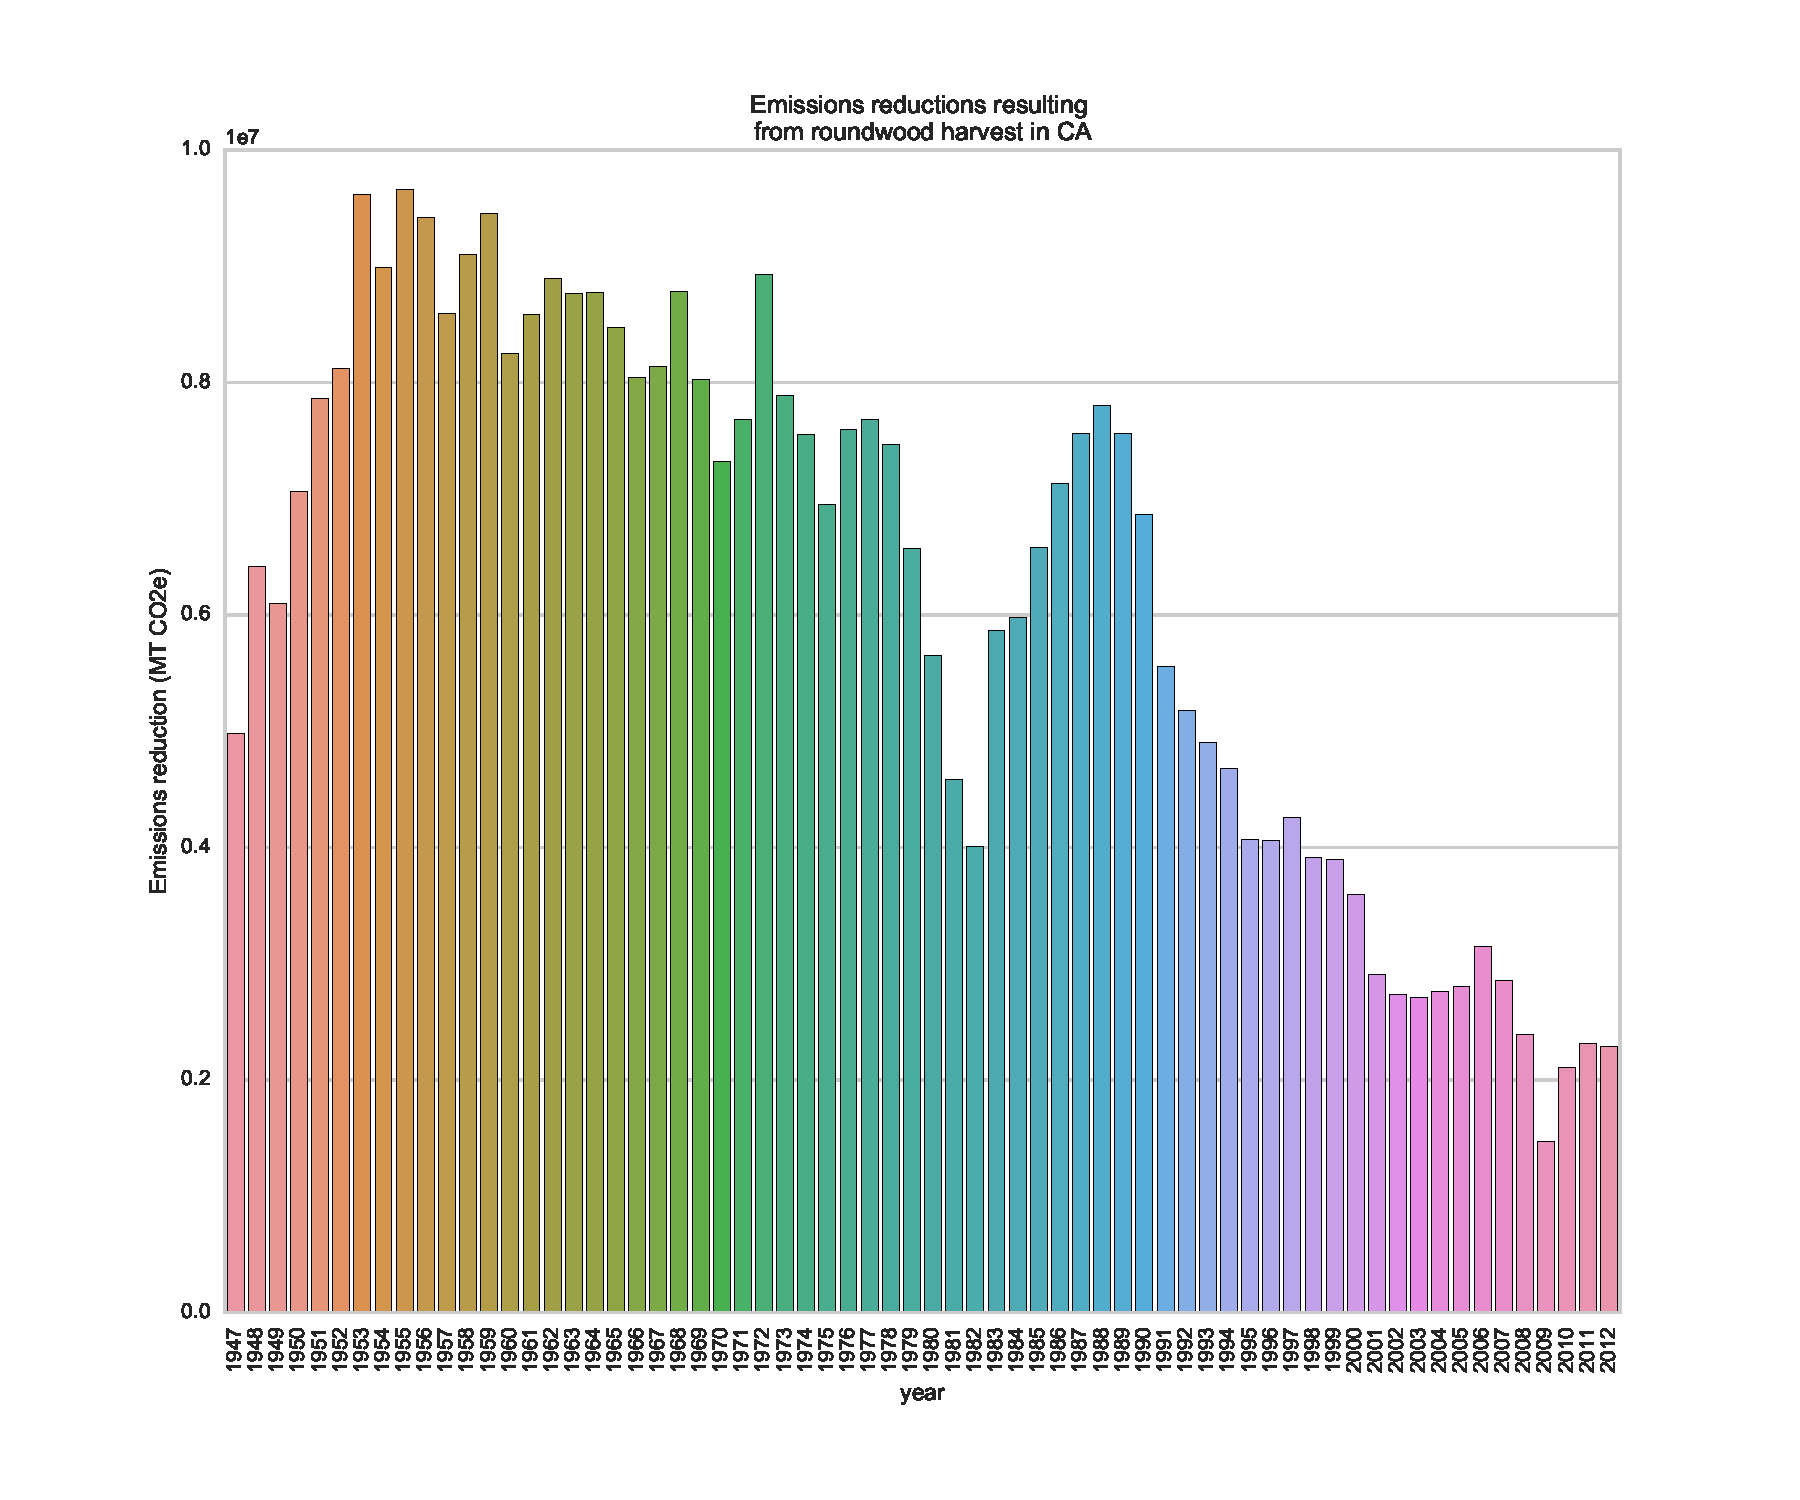
\includegraphics[width=\textwidth]{./graphics/ann_hh_em_reduc.pdf}
\caption{Historical emissions reductions resulting from harvested roundwood using displacement factors from \citep{Sathre2010} applied to TPO data.\label{em_reduc_hist}}
\end{figure}

Contribution of the varios ownership categories to the aggregate is
shown in Figure \ref{em_reduc_own}.

\begin{figure}[htb]
\centering
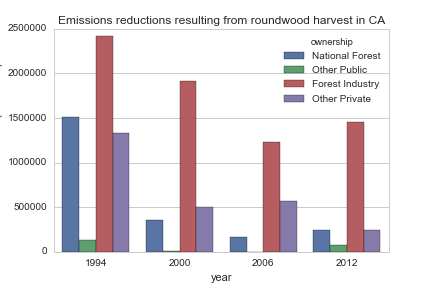
\includegraphics[width=.9\linewidth]{./graphics/harv_em_reductions.png}
\caption{\label{fig:orgparagraph1}
Historical emissions reductions by ownership for selected years resulting from harvested roundwood using displacement factors from \citep{Sathre2010} applied to TPO data. \label{em_reduc_own}}
\end{figure}

\section{Further Questions}
\label{sec:orgheadline21}

This analysis is a first step towards a broader analysis of the
climate impacts of harvested wood in California. The following are key
questions which follow from this analysis.

\section{References}
\label{sec:orgheadline22}
\bibliographystyle{IEEEtranSN}
\bibliography{fcat}
\end{document}